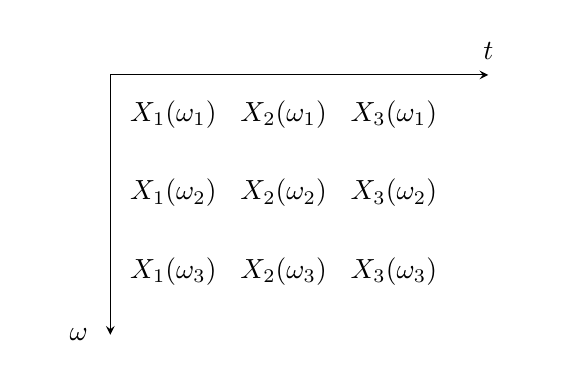
\begin{tikzpicture}[scale = 0.20]
    \definecolor{FFFFFF}{RGB}{255,255,255}
    \draw [draw=none] (37.0,-25.0) rectangle node(IDOL_J-3)[align = center, text width = 1.3 cm,inner sep=0] {$t$} (43.0,-28.0);
    \draw [draw=none] (11.0,-43.0) rectangle node(IDOL_J-4)[align = center, text width = 1.3 cm,inner sep=0] {$\omega$} (17.0,-46.0);
    \draw [draw=none] (17.0,-29.0) rectangle node(IDOL_J-5)[align = center, text width = 1.3 cm,inner sep=0] {$X_1(\omega_1)$} (23.0,-32.0);
    \draw [draw=none] (17.0,-34.0) rectangle node(IDOL_J-6)[align = center, text width = 1.3 cm,inner sep=0] {$X_1(\omega_2)$} (23.0,-37.0);
    \draw [draw=none] (17.0,-39.0) rectangle node(IDOL_J-7)[align = center, text width = 1.3 cm,inner sep=0] {$X_1(\omega_3)$} (23.0,-42.0);
    \draw [draw=none] (24.0,-29.0) rectangle node(ID_J-10)[align = center, text width = 1.3 cm,inner sep=0] {$X_2(\omega_1)$} (30.0,-32.0);
    \draw [draw=none] (24.0,-39.0) rectangle node(ID_J-12)[align = center, text width = 1.3 cm,inner sep=0] {$X_2(\omega_3)$} (30.0,-42.0);
    \draw [draw=none] (31.0,-29.0) rectangle node(ID_J-13)[align = center, text width = 1.3 cm,inner sep=0] {$X_3(\omega_1)$} (37.0,-32.0);
    \draw [draw=none] (31.0,-34.0) rectangle node(ID_J-14)[align = center, text width = 1.3 cm,inner sep=0] {$X_3(\omega_2)$} (37.0,-37.0);
    \draw [draw=none] (31.0,-39.0) rectangle node(ID_J-15)[align = center, text width = 1.3 cm,inner sep=0] {$X_3(\omega_3)$} (37.0,-42.0);
    \draw [draw=none] (24.0,-34.0) rectangle node(ID_J-23)[align = center, text width = 1.3 cm,inner sep=0] {$X_2(\omega_2)$} (30.0,-37.0);
    \draw [-stealth,solid](16.0,-28.0)--(40.0,-28.0);
    \draw [-stealth,solid] (16.0,-28.0) -- (16.0,-44.5);
\end{tikzpicture}
